\documentclass[12pt]{exam}

\newcommand{\course}{MTH 234 Summer 2021}
\newcommand{\qdate}{14.1 Group work } %PUT DATE HERE
\newcommand{\quiz}{Group Work} 

    \usepackage[top=1in, bottom=1in, left=.45in, right=.45in]{geometry}
    \usepackage{amsmath,amsthm,amssymb,amstext}
    \usepackage{enumerate,enumitem}
    \usepackage{tikz,float,graphicx}
    \usepackage{microtype}
    \usepackage{bm,tikz}
        \usetikzlibrary{calc,positioning}
    \usepackage{multicol}
    \usepackage{nicematrix}
    \usepackage{cleveref}
    \usepackage[framemethod=tikz]{mdframed}
    \usepackage{graphicx}
    \usepackage[export]{adjustbox}
    
    %\newcommand{\course}{MTH 234 Summer 2021}
    %\newcommand{\qdate}{Equations of lines and planes} %PUT DATE HERE
    %\newcommand{\quiz}{Group Work} 
    
    \newcommand{\R}{\mathbb{R}}
    
    \newcommand{\ba}{\bm{a}}
    \newcommand{\bb}{\bm{b}}
    \newcommand{\bc}{\bm{c}}
    \newcommand{\bi}{\bm{i}}
    \newcommand{\bj}{\bm{j}}
    \newcommand{\bk}{\bm{k}}
    \newcommand{\br}{\bm{r}}
    \newcommand{\bv}{\bm{v}}
    \newcommand{\bu}{\bm{u}}
    \newcommand{\gen}[1]{\left\langle #1 \right\rangle}
    \newcommand{\pd}[2]{\dfrac{\partial #1}{\partial #2}}

\newtheorem*{theorem}{Theorem}
\surroundwithmdframed[]{theorem}

\theoremstyle{definition}
    \newtheorem*{definition}{Definition}
    \surroundwithmdframed[]{definition}
    \newtheorem*{info}{Useful Information}
    \surroundwithmdframed[]{info}
\theoremstyle{remark}
    \newtheorem*{remark}{Remark}
    \surroundwithmdframed[]{remark}
    

%%%%%%%%%%%%%%%%%%%%%%%
% HEADER AND FOOTER
%%%%%%%%%%%%%%%%%%%%%%%
\pagestyle{headandfoot}
\firstpageheadrule
\runningheadrule
\firstpageheader{\course}{\quiz}{\qdate}
\runningheader{\course}{\quiz}{\qdate}
\runningfooter{}{}{}


\usepackage{color}
\shadedsolutions
\definecolor{SolutionColor}{rgb}{0.8,0.9,1}

\usepackage{pgfplots}
    \pgfplotsset{every axis/.append style={
                    axis x line=middle,    % put the x axis in the middle
                    axis y line=middle,    % put the y axis in the middle
                    axis z line=middle,
                    axis line style={<->}, % arrows on the axis
                    xlabel={$x$},          % default put x on x-axis
                    ylabel={$y$},          % default put y on y-axis
                    zlabel={$z$},
                    grid=both,
                    %xtick={-4,...,-1,1,...,3},
                    %ytick={-1,1,}
    }}
    \pgfplotsset{compat=1.17}

\newcommand{\bif}{\quad\iff\quad}

\printanswers
%\noprintanswers

\begin{document}

\section*{\qdate}


\subsection*{14.1: Functions of multiple variables}

\begin{questions}

\question Find and sketch the domain of \(f(x,y)=\dfrac{\sqrt{9-x^2-y^2}}{\sqrt{x^2+y^2-4}}\)
\ifprintanswers
        \begin{solution}
            The domain for this function is everywhere that
            \[
                9-x^2-y^2\ge 0 \quad \text{and}\quad x^2+y^2-4>0
            \]
            which is equivalent to 
            \[
                x^2+y^2\le 9 \quad \text{and}\quad x^2+y^2>4
            \]
            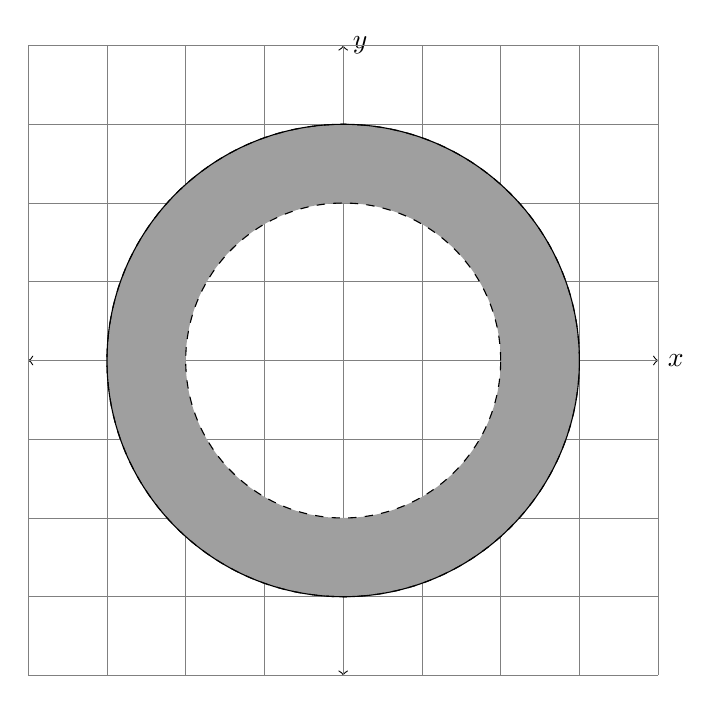
\begin{tikzpicture}
                \draw[<->,thin] (-4,0)--(4,0) node[right] {$x$};
                \draw[<->,thin] (0,-4)--(0,4) node[right] {$y$};
                \draw[very thin,gray] (-4,-4) grid (4,4) ;
                \draw[dashed,fill=gray!75,even odd rule] (0,0) circle[radius=3] (0,0) circle[radius=2];
                \draw (0,0) circle[radius=3];

            \end{tikzpicture}
        \end{solution}
    \else
        \vfill
    \fi

\question Let \(f(x,y)=\sqrt{x^2+y^2}.\)
\begin{parts} 
\part What is the domain of \(f(x,y)\)?
    \ifprintanswers
        \begin{solution}
        \(f(x,y)\) is defined as long as \(x^2+y^2\ne 0\), which means everywhere except the point \((0,0)\), i.e. \(\{(x,y)\in\R^2~~|~~(x,y)\ne (0,0)\}\).
        \end{solution}
    \else
        \vspace{1cm}
    \fi
\part Sketch a contour plot for \(f(x,y)\) using level curves \(f(x,y)=k\) for 
\(k=0,1,2,3,4,5\).

\ifprintanswers
        \begin{solution}
         \begin{center}
        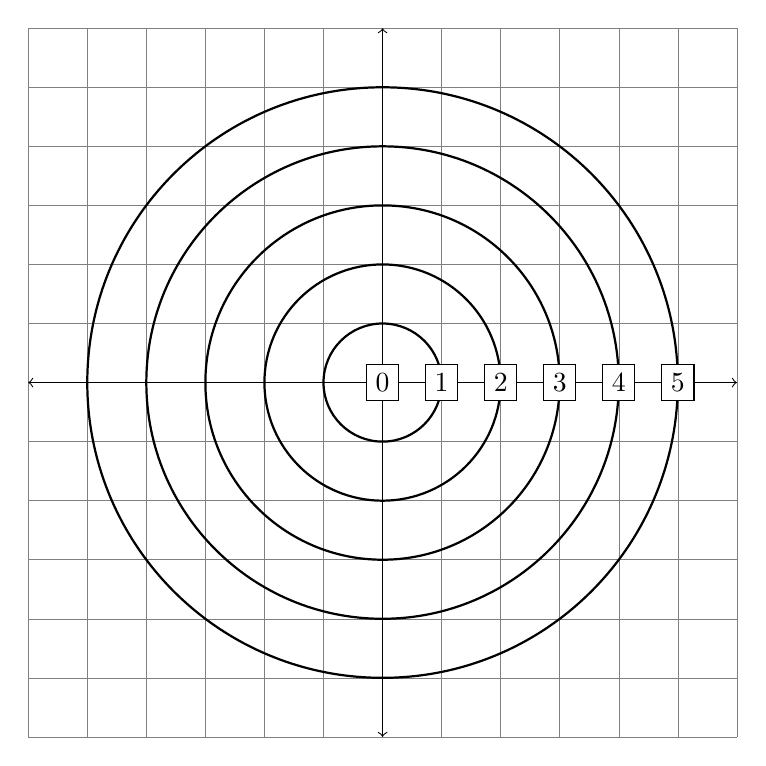
\begin{tikzpicture}[scale=.75]
            \draw[very thin, gray] (-6,-6) grid (6,6);
            \draw[thin,<->] (-6,0)--(6,0);
            \draw[thin,<->] (0,-6)--(0,6);

            \foreach \k in {1,2,3,4,5}
            {

                \draw[thick] (0,0) circle[radius=\k];
            }
            \foreach \x in {0,1,2,3,4,5}{
                \node[draw,fill=white] at (\x,0) {$\x$};
            }
            
        \end{tikzpicture}
        \end{center}
        \end{solution}
    \else
        \vfill
    \fi
    \part 
    Use the above to sketch \(f(x,y)\). Illustrate the curves cooresponding to curves drawn in the contour plot above.
    \ifprintanswers
        \begin{solution}
        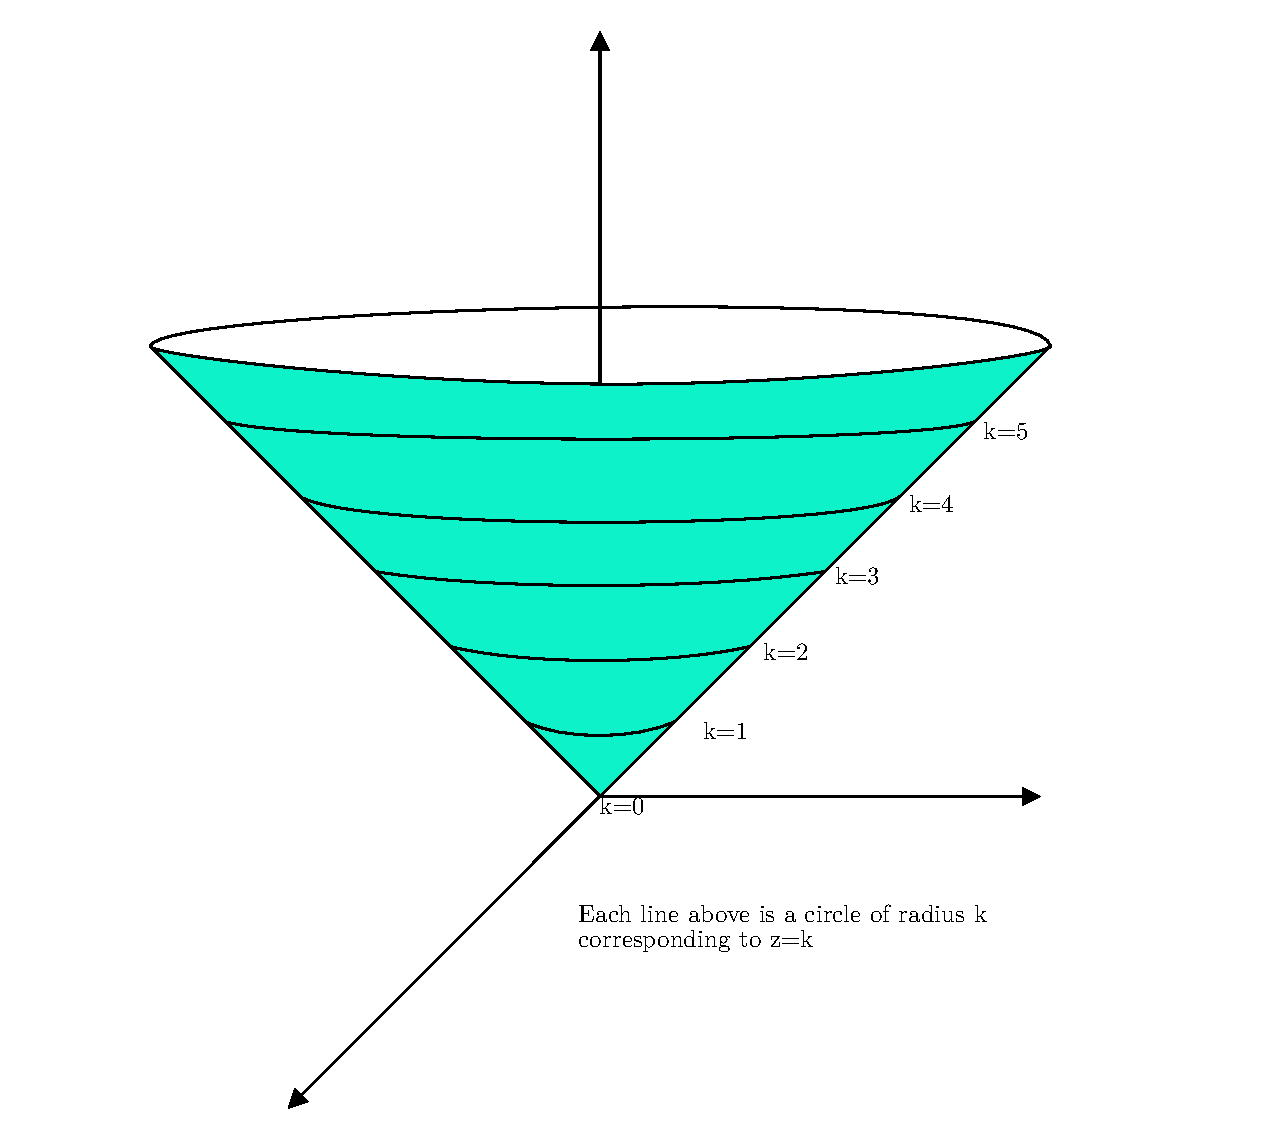
\includegraphics[width=.75\textwidth]{cone_with_curves.pdf}
        \end{solution}
    \else
        \vfill
    \fi
\end{parts}


\end{questions}

\end{document}

%soln : Question environment
    \ifprintanswers
        \begin{solution}
        \end{solution}
    \else
        \vfill
    \fi